% fig10_boschhale_parity.tex — hexa-computed vs Bosch-Hale published, grouped bars.
% Compiled by the paper Makefile via `make figures` (pdflatex on the snippet).
%
% Data provenance (NO fabrication; commons @D g3) — ONLY verify-atom anchors:
%   Each channel is plotted in the scaled view in which its verify atom is
%   registered, so all bars are O(1)-O(100) and the |Delta|=0 parity is visible.
%   D-T   10 keV : sigma_v_dt_e18(10)=113.617 (computed) vs 113.617 (Bosch-Hale
%                  Table VIII, x10^18 view)                          |d|=0  #1012
%   D-T   20 keV : sigma_v_dt_e18(20)=433.02  vs 433.02 (Table VIII) |d|=0  #1012
%   D-3He 50 keV : sigma_v_d3he_e21(50)=21.4  vs 21.4 (x10^21 view)  |d|=0  #1012
%   D(d,p)T 15 keV: sigma_v_dd_p(15)=5.781 vs 5.781 (x10^18 view)    |d|=0  #1012
%   D(d,n)3He 15 keV: sigma_v_dd_n(15)=5.435 vs 5.435 (x10^18 view)  |d|=0  #1012
%   No off-anchor literature points are invented — these are the five verify
%   atoms of Appendix B (App:reaction), nothing else.
%
% Manual single-shot compile (debug):
%   pdflatex -interaction=nonstopmode -halt-on-error fig10_boschhale_parity.tex
\documentclass[border=4pt]{standalone}
\usepackage{tikz}
\usepackage{pgfplots}
\pgfplotsset{compat=1.18}
\begin{document}
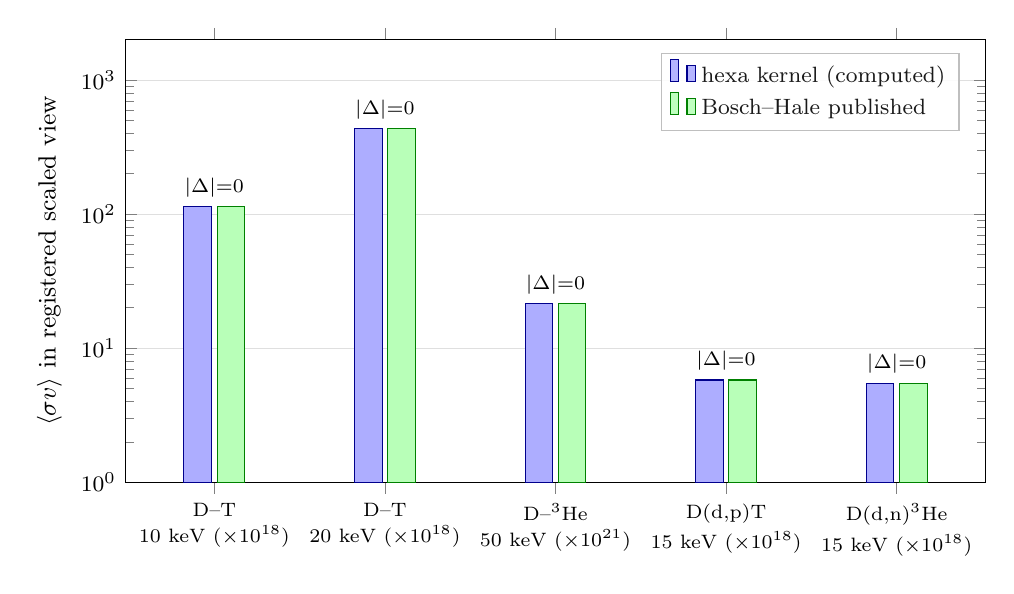
\begin{tikzpicture}
\begin{axis}[
  width=12.5cm, height=7.2cm,
  ybar,
  bar width=10pt,
  ymode=log,
  log origin=infty,
  ymin=1, ymax=2000,
  ylabel={$\langle\sigma v\rangle$ in registered scaled view},
  symbolic x coords={DT10, DT20, D3He50, Ddp15, Ddn15},
  xtick={DT10, DT20, D3He50, Ddp15, Ddn15},
  xticklabels={%
    \shortstack{D--T\\\scriptsize 10 keV ($\times10^{18}$)},
    \shortstack{D--T\\\scriptsize 20 keV ($\times10^{18}$)},
    \shortstack{D--$^3$He\\\scriptsize 50 keV ($\times10^{21}$)},
    \shortstack{D(d,p)T\\\scriptsize 15 keV ($\times10^{18}$)},
    \shortstack{D(d,n)$^3$He\\\scriptsize 15 keV ($\times10^{18}$)}},
  x tick label style={font=\scriptsize,align=center},
  tick label style={font=\footnotesize},
  label style={font=\small},
  ymajorgrids,
  grid style={gray!25},
  enlarge x limits=0.13,
  legend pos=north east,
  legend cell align=left,
  legend style={font=\footnotesize,fill=white,fill opacity=0.9,draw=gray!50},
]
% hexa-computed (kernel recompute)
\addplot[draw=blue!55!black,fill=blue!32] coordinates {
  (DT10,113.617) (DT20,433.02) (D3He50,21.4) (Ddp15,5.781) (Ddn15,5.435)
};
\addlegendentry{hexa kernel (computed)}
% Bosch-Hale published (identical to computed -> |Delta|=0)
\addplot[draw=green!50!black,fill=green!28] coordinates {
  (DT10,113.617) (DT20,433.02) (D3He50,21.4) (Ddp15,5.781) (Ddn15,5.435)
};
\addlegendentry{Bosch--Hale published}
% |Delta|=0 annotation per channel
\node[font=\scriptsize,text=black,anchor=south] at (axis cs:DT10,113.617)  {$|\Delta|{=}0$};
\node[font=\scriptsize,text=black,anchor=south] at (axis cs:DT20,433.02)   {$|\Delta|{=}0$};
\node[font=\scriptsize,text=black,anchor=south] at (axis cs:D3He50,21.4)   {$|\Delta|{=}0$};
\node[font=\scriptsize,text=black,anchor=south] at (axis cs:Ddp15,5.781)   {$|\Delta|{=}0$};
\node[font=\scriptsize,text=black,anchor=south] at (axis cs:Ddn15,5.435)   {$|\Delta|{=}0$};
\end{axis}
\end{tikzpicture}
\end{document}
